\section{Base Model}
First, we set out to develop a base model. However, first, we had to decide which image size to use.
We chose an image size of 224 by 224, since almost all images are bigger on each axis, so we almost only shrink pictures.
The pretrained models also uses resizing to 224 pixels making our model more comparable to the pretrained ones.
Resizing the images has the effect of reducing the size of the input to the model which will reduce the accuracy a little bit, but make it train significantly faster.

Next, we had to decide how many layers our model should have.
As the task is relatively simple, we decided to use 4 convolutional layers and 3 fully connected layers.
Since the input images are in color and 224 pixels on each axis, inputting that image directly into the fully connected layers would result in a 224*224*3 = 150528 input size into the model. We would like to reduce this further, so the fully connected layers does not get an input of 150528. The convolution layers extract features, which makes it possible for the neural network to recognise a specific feature no matter where it is in the image, instead of having to learn that feature for every possible position in an image.

We use cross entropy loss as our loss function since this loss function is a popular and good loss function for classification tasks. We use adam as the optimizer since it combines the strength of several other optimizers. 


The base model is shown in Table \ref{tab:base_model}.
\begin{table}[H]
    \vspace*{-0.5cm}
    \centering
    \begin{tabular}{|l|c|c|c|c|}
    \hline
                & \textbf{Output}           & \textbf{Kernel}   & \textbf{MaxPooling}   & \textbf{Activation}   \\ 
                & \textbf{kernels/features} &                   &   &   \\ \hline
    Conv2D w/   & 32                        & 3x3                   & 2x2                   & ReLU                  \\ \hline
    Conv2D w/   & 64                        & 3x3                   & 2x2                   & ReLU                  \\ \hline
    Conv2D w/   & 128                       & 3x3                   & 2x2                   & ReLU                  \\ \hline
    Conv2D w/   & 256                       & 3x3                   & 2x2                   & ReLU                  \\ \hline
    Linear w/   & 256                       & -                     & -                     & ReLU                  \\ \hline
    Linear w/   & 128                       & -                     & -                     & ReLU                  \\ \hline
    Linear w/   & 2                         & -                     & -                     & -                     \\ \hline
    \end{tabular}
    \caption{Base Model.}
    \label{tab:base_model}
    \vspace*{-0.8cm}
\end{table}
Results of the base model after 25 epochs are shown in Figure \ref{fig:base_model_results}.
\begin{figure}[H]
    \vspace*{-0.7cm}
    \centering
    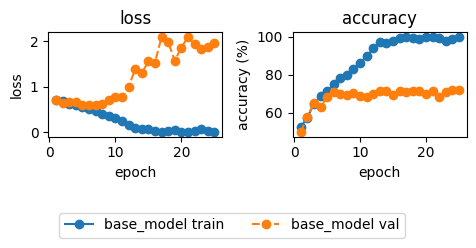
\includegraphics[width=0.4\textwidth]{figures/results_base_model.png}
    \caption{Base Model Results.}
    \label{fig:base_model_results}
    \vspace*{-0.7cm}
\end{figure}

We chose to train the model in 100 epochs. This is a sufficiently high number that the model gets to be properly trained, but still a reasonable number to keep within a reasonable time to train the model. More epochs is good until a certain point when the model starts overfitting. As an improvement we could have included some early stopping in case the model began overfitting.
We chose a learning rate of 0.001. A learning rate that is too small could result in a very slow learning process that might get stuck, and a too big learning rate could result in learning a suboptimal set of weights or an unstable learning process. A smaller learning rate requires more epochs for a better result. The default learning rate is 0.01. We chose a smaller learning rate since we wanted our learning process to be very stable, and since we run 100 epochs it seemed appropriate.

Clearly, the base model is overfitting, one way, especially for small datasets as in this case, to reduce overfitting is to use data augmentation, enabling the model to learn from more data.
